\section{Compiler}\label{sec:compiler}

Damit eine Programmiersprache praktisch einsetzbar ist, muss sie nicht nur in Syntax und Semantik definiert sein, sondern auch ausführbar sein.
Dies kann einerseits durch direktes Ausführen des Programmtexts geschehen, wie es beispielsweise bei Skriptsprachen der Fall ist.
Andererseits kann eine Programmiersprache auch in ein maschinenlesbares Format übersetzt werden, das dann direkt oder durch eine virtuelle Maschine ausgeführt wird.
Dieser Ansatz nennt sich Kompilierung.
In Java wird sie durch den Java Compiler durchgeführt, der Bytecode erzeugt.
Dieser kann von einer \ac{jvm} ausgeführt werden.

Scenarios werden in zwei Schritten ausführbar gemacht.
Zunächst werden deren Quelltexte durch den Scenario-Compiler in Java-Quellcode übersetzt.
Der entstehende Quellcode wird dann vom Java-Compiler in ausführbaren Bytecode kompiliert, der letzlich von einer \ac{jvm} ausgeführt werden kann.
Dieses Vorgehen wurde der direkten Ausführung vorgezogen, da der Java-Code als Zwischenergebnis einerseits dem Verständnis durch Vertrautheit dient und andererseits die Anpassung und Erweiterung um Aspekte erlaubt, für welche die Scenario-Sprache nicht vorgesehen ist.
Die Architektur und Implementierung des Scenario-Compilers sind Inhalt dieses Abschnitts.
Dabei wird des Öfteren auf das Beispiel in Listing~\ref{lst:CompilationExample.md} Bezug genommen, dessen Übersetzung bis zum Java-Quellcode in den einzelnen Teilabschnitten stückweise erarbeitet wird.

\begin{listing}[htp]
    \centering
    \code{src/main/scenarios/org/example/CompilationExample.md}
    \inputminted{md}{chapter/fulib-scenarios/scenarios/CompilationExample.md}
    \vspace{-3ex}
    \caption{Beispiel-Scenario zur Demonstration des Scenario-Compilers}
    \label{lst:CompilationExample.md}
\end{listing}

\subsection{Architektur}\label{subsec:compiler-architecture}

Die Kompilierung von Programmiersprachen ist eine komplexe Aufgabe, bei der viele Schritte zusammenwirken müssen und zum Ergebnis beitragen.
Deshalb ist es wichtig, dass ein Compiler sie in einer übersichtlichen Architektur aufbaut.
Die Schritte werden auch als \emph{Phasen}\cite[S.~4]{dragonbook} bezeichnet.
Im Groben kann der Scenario-Compiler in drei Phasen unterteilt werden, deren Aufgaben sich stark unterscheiden.

Die erste Phase ist das Frontend, das für das Einlesen und Strukturieren von Quelltext zuständig ist.
Es kann einen zusammenhängenden Text als Folge von Wörtern, Ausdrücken und Sätzen verstehen, und daraus anhand der Regeln der Sprache einen Baum bilden, der die Struktur des Texts abbildet.
Dafür muss der Quelltext die Grammatik der Sprache befolgen, andernfalls ist das Frontend für die Ausgabe von Fehlermeldung zuständig, die auf Unstimmigkeiten im Text hindeuten.

Die Verarbeitung dieses Baumes ist dann Aufgabe der Analyse- und Transformationsphase, welche die zweite Phase darstellt\footnote{Aufgrund des großen Umfangs wird sie hier als eigenständig und nicht als Teil des Frontends aufgefasst.}.
Dabei wird der Baum anhand von Regeln, die aus der Semantik der Sprache hervorgehen, umgeformt und geprüft.
Zur Analyse gehört ferner die Diagnose von Problemen, die über einfache Syntaxfehler hinausgehen.
Ergebnis der Phase ist eine neue Baumstruktur, die auf der vom Frontend stammenden aufbaut, sie aber um zusätzliche Informationen erweitert oder teilweise vereinfacht.

Die letzte Phase wird als Backend bezeichnet.
Dessen Aufgabe ist es, Code in einer Zielsprache anhand des Ergebnisses der Analyse zu generieren.
Im Fall des Scenario-Compilers ist Java die Zielsprache, jedoch wären auch andere Programmier- oder Maschinensprachen möglich.
Das Backend kennt dabei die Details zum Aufbau der Zielsprache  und definiert Regeln zur Übersetzung der Baumstruktur.

Die drei Phasen sowie deren Unterphasen sind in Abbildung~\ref{fig:compiler-architecture} dargestellt.
Sie dient als Referenz für die folgenden Unterabschnitte, in denen die Phasen und ihre Unterteilung im Detail erläutert werden.

\begin{figure}
    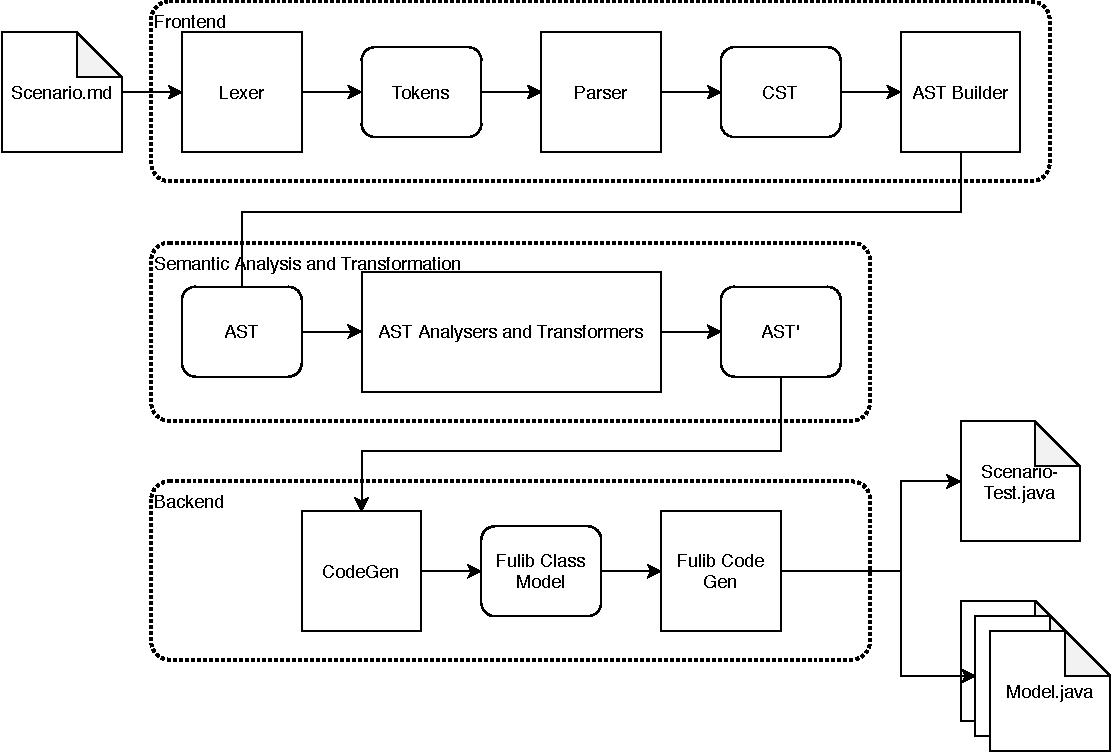
\includegraphics[width=\textwidth]{chapter/fulib-scenarios/img/architecture.pdf}
    \caption{Compiler-Architektur}
    \label{fig:compiler-architecture}
\end{figure}

\subsection{Frontend}\label{subsec:frontend-antlr4}

Die Übersetzung der Markdown-Datei beginnt mit deren Einlesen und Umwandeln in verarbeitbare Daten.
Im Compilerbau wird dies klassisch in zwei Schritte unterteilt.
Der \emph{Lexer} wandelt die Zeichenfolge in eine Liste von Wörtern mit Typinformationen, genannt \emph{Tokens}, um.
Dann bringt der \emph{Parser} die flache Liste von Tokens nach den Regeln der Grammatik in eine Baumstruktur, die \acfi{cst} genannt wird.

Da die Umwandlung in Tokens und deren Strukturierung in den meisten Compilern Anwendung findet und deren Implementierung meist nach einem festen Muster stattfindet, existieren Tools, welche diesen Prozess vereinfachen.
Diese werden \emph{Compiler-Compiler} oder \emph{Lexer-} und \emph{Parsergeneratoren} genannt.

Das Frontend des Scenario-Compilers basiert auf dem Parsergenerator ANTLR~4~\cite{antlr4-reference}.
Mit diesem können Grammatiken in einem Format spezifiziert werden, das einer formalen Grammatik für reguläre und kontextfreie Sprachen ähnelt.
Daraus generiert das Tool dann Java-Code, der Dateien einlesen kann und daraus einen \ac{cst} generiert.

Zunächst soll betrachtet werden, wie die FulibScenarios-Grammatik definiert ist.
Diese ist für Lexer und Parser getrennt.
In Listing~\ref{lst:ScenarioLexer.g4} ist ein Ausschnitt der ANTLR-Grammatik zu sehen, welche den Lexer definiert.
Der Ausschnitt ist ausreichend, um das Scenario aus Listing~\ref{lst:CompilationExample.md} verarbeiten zu können.
Die eigentliche Grammatik von FulibScenarios besteht aus vielen weiteren Regeln, um alle Funktionen der Sprache zu implementieren.
Sie ist unter~\cite{lexer-grammar} zu finden.

\codelisting{antlr}{chapter/fulib-scenarios/grammars}{ScenarioLexer.g4}{Ausschnitt der Scenario-Lexer-Grammatik}

Die Grammatik besteht aus mehreren Regeln, die einem Muster einen Namen zuordnen.
Dieser Name wird später den Tokens zugeordnet.
So haben Tokens mit dem Text \code{and} später den Namen \code{AND} und jene, die ein Wort darstellen, den Namen \code{WORD}.
Im Folgenden werden Tokens mit der Kurzschreibweise \code{<name>(<text>)} bezeichnet, beispielsweise \code{AND(and)} und \code{WORD(Alice)}.

Die rechte Seite jeder Regel ähnelt einem regulären Ausdruck.
Bei Schlüsselwörtern wie \code{a}, \code{is} und \code{with} muss der Text exakt der vorgegebenen Schreibweise entsprechen, während \code{There} beispielsweise auch kleingeschrieben werden kann.
Ein \code{HEADLINE}-Token entsteht, wenn auf ein \code{#}-Zeichen beliebig viele Zeichen und ein Zeilenumbruch folgen.
Wörter beginnen mit einem Buchstaben, gefolgt von beliebig vielen Buchstaben, Ziffern, Apostrophen, Unterstrichen und Bindestrichen.
Die Regel \code{WS} sorgt durch die Angabe \code{-> skip} dafür, dass Whitespace-Zeichen nicht zu Token werden.
Falls mehrere Regeln infrage kommen würden, wird zunächst die längstmögliche Übereinstimmung angewandt;
falls das nicht eindeutig bestimmbar ist, wird die als erste definierte Regel bevorzugt.
So wird aus dem Text \code{ampersand} nicht die Token-Folge \code{A(a), WORD(mpers), AND(and)}, sondern \code{WORD(ampersand)}.

Wendet man die Regeln aus Listing~\ref{lst:ScenarioLexer.g4} auf das Scenario aus Listing~\ref{lst:CompilationExample.md} an, so erhält man die in Listing~\ref{lst:CompilationExampleTokens.txt} gezeigte Liste von Tokens.

\codelisting{text}{chapter/fulib-scenarios/trees}{CompilationExampleTokens.txt}{Aus Listing~\ref{lst:CompilationExample.md} abgeleitete Token-Liste}

Als Nächstes sollen diese Tokens in einen \ac{cst} umgewandelt werden.
Dies ist die Aufgabe des Parsers.
Listing~\ref{lst:ScenarioParser.g4} zeigt einen für das Beispiel-Scenario ausreichenden Ausschnitt der Grammatik, die den Parser definiert.
Die vollständige Parser-Grammatik ist unter~\cite{parser-grammar} auffindbar.

\codelisting{antlr}{chapter/fulib-scenarios/grammars}{ScenarioParser.g4}{Ausschnitt der Scenario-Parser-Grammatik}

Die Struktur der Parser-Grammatik ist ähnlich zur Lexer-Grammatik.
Wieder gibt es benannte Regeln, jedoch bestehen deren rechte Seite nicht aus regulären Ausdrücken, sondern aus \emph{Nicht-Terminal}-Symbolen, die weitere Parser-Regeln referenzieren\footnote{Diese sind in der ANTLR-Grammatik daran zu erkennen, dass sie mit einem Kleinbuchstaben beginnen.}, sowie \emph{Terminal}-Symbolen, die analog Verweise auf Lexer-Regeln sind\footnote{In ANTLR beginnen diese immer mit einem Großbuchstaben.}.
Die \code{thereSentence}-Regel aus Listing~\ref{lst:ScenarioParser.g4} beginnt beispielsweise mit den Terminalen \code{THERE}, \code{IS}, \code{A} und \code{WORD}, gefolgt von dem Nicht-Terminal \code{withClause}.
Beim Ableiten eines konkreten Syntaxbaumes werden alle Terminale zu den Blättern, während die Nicht-Terminale zu Elternknoten werden.

In Listing~\ref{lst:ScenarioParser.g4} dient \code{file} als Startregel.
Nun wird diese Regel \emph{abgeleitet}, indem entweder die Tokens, die derzeit am Anfang der Token-Liste stehen, einem Terminal zugeordnet werden, oder ein Nicht-Terminal rekursiv abgeleitet wird.
Da \code{file} mit dem Nicht-Terminal \code{header} beginnt, wird zunächst dieses abgeleitet.
Dabei wird dem Terminal \code{HEADLINE} das Token \code{HEADLINE(# My First Scenario)} zugeordnet.
Als Nächstes werden \code{sentence} und \code{thereSentence} abgeleitet, wobei den Terminalen \code{THERE}, \code{IS} und \code{A} und \code{WORD} das entsprechende Token zugeordnet wird.
Die Ableitung von \code{withClause} erfolgt durch einfache Zuweisung der drei nächsten Tokens zu den entsprechenden Terminalen.
Zuletzt wird der Punkt am Ende des Satzes dem \code{FULL_STOP}-Terminal zugeordnet.

Nun sind alle Token, die der Lexer aus der Eingabe produziert hat, verbraucht, und der Parse-Vorgang ist abgeschlossen.
Das Ergebnis ist der in Abbildung~\ref{fig:parsetree} sichtbare Syntaxbaum.

\begin{figure}
    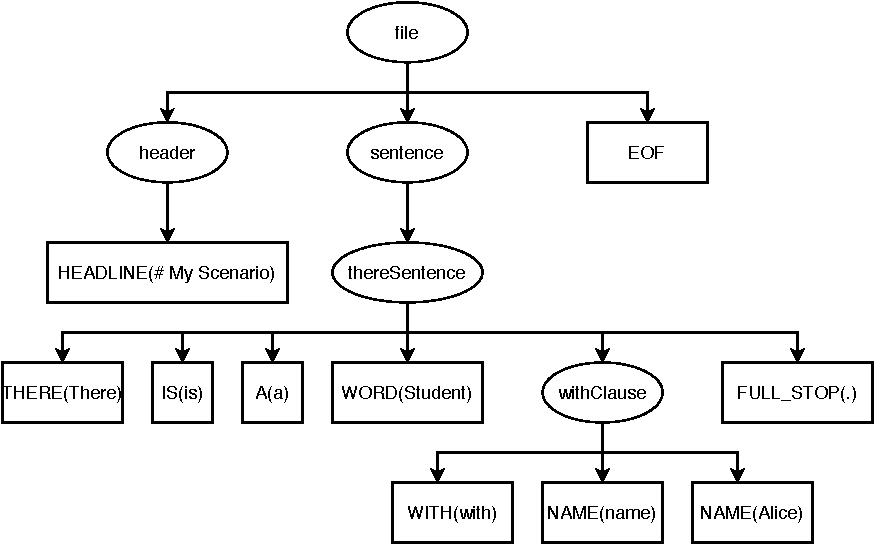
\includegraphics[width=\textwidth]{chapter/fulib-scenarios/img/parsetree.pdf}
    \caption{Syntaxbaum von Listing~\ref{lst:CompilationExample.md}}
    \label{fig:parsetree}
\end{figure}

Der \ac{cst} ist eng an die Struktur der Grammatik gebunden.
Bei Änderungen an der Grammatik, beispielsweise dem Einfügen von gemeinsam genutzten Hilfsregeln beim Refactoring, ändert sich auch die Struktur des \ac{cst}.
Würde man den \ac{cst} für weitere Schritte des Compile-Vorgangs verwenden, müsste die Implementierung dieser Schritte bei Änderung der Grammatik an die neue \ac{cst}-Struktur angepasst werden, was zu einem Wartungsproblem führt.
Deshalb hat das Frontend zusätzlich die Aufgabe, den \ac{cst} in eine umgänglichere Form umzuwandeln.
Diese wird \acfi{ast} genannt.

Der \ac{ast} besteht aus einem weiteren Datenmodell, das vollständing von dem für den Parser verwendeten getrennt ist.
Während letzteres von ANTLR aus der Grammatik hergeleitet und generiert wird, ist das Datenmodell des \ac{ast} manuell definiert und am logischen Aufbau eines Szenarios orientiert.
So gibt es \ac{ast}-Klassen für Pakete, Dateien, Scenarios in Dateien und jegliche Arten von Sätzen und Ausdrücken.
Für bestimmte Konstrukte, die in mehreren Sätzen vorkommen, gibt es Hilfsklassen, die Code-Duplizierung vermeiden.
Dazu gehören z.B.\ mit Namen versehene Ausdrücke.

Das Datenmodell des \ac{ast} wird ebenfalls automatisch generiert.
Grund dafür ist, dass jede \ac{ast}-Klasse lediglich aus Klassenvariablen, Gettern und Settern sowie einer Factory-Methode besteht.
Diese können mit einer Liste von Attributen ausreichend definiert werden.
Die Generierung des \ac{ast} erfolgt durch das von mir entwickelte GenTreeSrc-Tool~\cite{gentreesrc}.
Dieses erlaubt die Definition von Klassen und Attributen in einer \code{gts}-Datei, aus der dann Java-Dateien generiert werden können.
Listing~\ref{lst:FulibScenarios1.gts} zeigt einen Ausschnitt der \code{gts}-Datei von FulibScenarios, in dem die für Beispiel~\ref{lst:CompilationExample.md} benötigten Definitionen abgebildet sind.
Die vollständige Definitionsdatei ist unter~\cite{gts-definitions} zu finden.

\codelisting{java}{chapter/fulib-scenarios/definitions}{FulibScenarios1.gts}{Ausschnitt der FulibScenarios.gts-Datei}

Die Definitionsdatei verwendet die Syntax von GenTreeSrc, die wie folgt zu lesen ist:
Auf der obersten Ebene werden Klassen inkl.\ Package-Name definiert, zum Beispiel \code{org.fulib. scenarios.ast.Node}. % manual line break
Das Schlüsselwort \code{abstract} bedeutet hier, dass diese ein Interface ist und nicht instanziiert werden kann.
In den geschweiften Klammern nach einer Klassendefinition werden weitere Klassen definiert, die von dieser erben sollen.
So erbt beispielsweise \code{ScenarioFile} von \code{Node} und gehört ebenfalls zum Package \code{org.fulib.scenarios.ast}.
Relative Package-Namen wie \code{decl.Name} bewirken, dass die Klassen in einem Unterpackage relativ zu ihren Elternklassen ablegt werden, in diesem Fall wäre der qualifizierte Klassenname folglich \code{org.fulib.scenarios.ast.decl.Name}.
Runde Klammern nach dem Klassennamen enthalten die Attribute, welche die Syntax \code{name: Typ} verwenden.
Die Typausdrücke \code{[T]} und \code{[T:U]} stehen für \code{List<T>} und \code{Map<T, U>}.
Einfache Attribute haben einen Getter und, sofern nicht das Schlüsselwort \code{readonly} vorhanden ist, einen Setter.
Aus jedem Attribut wird ein Parameter im Konstruktor bzw.\ der Factory-Methode der generierten Klasse.

Mit den generierten Klassen kann nun ein \ac{ast} erzeugt werden.
Dafür implementiert das Frontend einen Übersetzungsschritt für eine Vielzahl von \ac{cst}-Knoten, der diese bei den Blättern beginnend in \ac{ast}-Knoten umwandelt.

Ergebnis der Übersetzung des in Abbildung~\ref{fig:parsetree} gezeigten \ac{cst} ist der \ac{ast}, der in Listing~\ref{lst:CompilationExampleAST.txt} in seinem Ausgabeformat dargestellt ist\footnote{
    Im Scenario-Compiler steht auf der obersten Ebene ein \code{CompilationContext}-Knoten, der unter anderem Kompilierungsoptionen enthält.
    Darunter befinden sich Knoten für Pakete;
    erst diese enthalten den \code{ScenarioFile}-Knoten.
    Aus Gründen der Einfachheit wurden diese beiden Ebenen hier ausgelassen.
}.

\codelisting{java}{chapter/fulib-scenarios/trees}{CompilationExampleAST.txt}{\ac{ast} von Listing~\ref{lst:CompilationExample.md}}

\subsection{Analyse und Transformation}\label{subsec:data-model-gentreesrc}

Sobald der \ac{ast} im Frontend erzeugt wurde, beginnt die Analyse- und Transformationsphase.
Deren Aufgabe ist es, den \ac{ast} auf semantische Gültigkeit zu überprüfen und ihn so vorzubereiten, dass in der folgenden Codegenerierungsphase alle Informationen bereitstehen.

Bei der Analyse werden die Fehler- und Warnmeldungen erzeugt, welche die Ausgabe des Compilers bilden.
Dafür werden im \ac{ast} durch das Frontend Positionsinformationen von Tokens hinterlegt, die es ermöglichen, in den Meldungen Dateinamen, Zeilen- und Spaltennummern einzubringen.
Die entsprechenden Attribute in \ac{ast}-Klassen wurden hier zur Einfachheit ausgelassen, sie sind jedoch unter~\cite{gts-definitions} vollständig erfasst.

Die Analyse- und Transformationphase besteht im Scenario-Compiler aus zwei logisch getrennten Unterphasen, der Gruppierung und der Namensauflösung.
Die Gruppierung ist zuständig dafür, aus der linearen Abfolge von Sätzen in einem Scenario eine Baumstruktur zur erzeugen, wenn Sätze anderen untergeordnet werden können.
Dies ist beispielsweise bei jenen Sätzen der Fall, die unter einem \code{Call}-Satz stehen, wie im vorherigen Abschnitt unter~\ref{subsec:methods} näher erläutert wurde.
Jeder Satz, dessen Subjekt dem des \code{Call}-Satzes entspricht, wird diesem untergeordnet und ist nicht länger Element der Satzliste des Scenarios.
Grund dafür ist, dass der Code für diese Sätze später nicht im Test, sondern in der entsprechenden Methode auftaucht.
Da für die Bestimmung von Subjekten keine komplexe Namensauflösung notwendig ist, die Unterordnung von Sätzen jedoch die Sichtbarkeit von Namen beeinflusst, geschieht die Gruppierung vor der Namensauflösung.

Die Namensauflösung umfasst mehrere Teilaufgaben:

\begin{itemize}
    \item Die direkte Auflösung und Erzeugung sichtbarer Variablen, Klassen und Methoden
    \item Die Auflösung und Erzeugung von Attributen, Assoziationen und Methoden in Klassen und dem dadurch definierten Namensraum
    \item Das Erzeugen von Diagnosenachrichten
    \item Die Umstrukturierung des \ac{ast}
\end{itemize}

Der Grund für die Zusammenfassung der Teilaufgaben ist, dass diese eng verzahnt und meist in einem Schritt ausführbar sind.
Beispielsweise beim Auflösen einer Assoziation kann diese angelegt werden, falls es sie noch nicht gibt, andernfalls muss die bestehene Assoziation mit der neuen Definition auf Konsistenz überprüft und ggf.\ eine Fehlermeldung erzeugt werden.
Diese kann zum Beispiel auftreten, wenn bei der zweiten Verwendung die Rückrichtung falsch benannt wird:

\begin{codeblock}
    Kassel has country and is one of the cities of Germany.
    Berlin has country and is the capital of Germany.
\end{codeblock}

Dies erzeugt die folgende Fehlermeldung in der Konsolenausgabe des Compilers:

\begin{codeblock}
    src/org/example/ErrorExample.md:4:30: error: conflicting redeclaration of reverse association of 'City.country' [association.reverse.conflict]
    was: Country.cities, association to many 'City'
    now: Country.capital, association to one 'City'
\end{codeblock}

Die Fehlermeldungen sind so strukturiert, dass sie alle nötigen Informationen zur Lösung des Problems enthalten.
Zu Beginn stehen Dateiname, Zeile und Spalte, die mit einer \ac{ide} direkt an der richtigen Stelle geöffnet werden können.
Nach der Angabe der Dringlichkeit der Meldung, die im Beispiel \code{error} ist, aber auch \code{syntax}, \code{warning} oder \code{note} sein könnte, folgt eine kurze Beschreibung der Problemursache.
In den eckigen Klammern steht eine feste Meldungs-ID, nach der beispielsweise in der Dokumentation, bei Google oder StackOverflow gesucht werden kann.
Dadurch kann auch die Formulierung der Beschreibung geändert oder in eine andere Sprache übersetzt werden, ohne dass Online-Suchen erschwert werden.
Viele (Fehler-)Meldungen enthalten außerdem einige Zeilen mit zusätzlichen Informationen, wie hier die Informationen zur vorherigen und jetzigen Deklaration der Assoziation.
Diese sollen den Entwickler ebenfalls bei der Problembehebung unterstützen.

Eine weitere Aufgabe der Transformationsphase ist es, den \ac{ast} vor der Auflösung zu vereinfachen.
Bildet man beispielsweise eine Art von \ac{ast}-Knoten immer auf eine andere ab, müssen folgende Schritte nicht mehr für die erste Knotenart implementiert werden, da man sichergehen kann, dass sie nicht mehr vorkommt.
Dadurch kann Codeduplizierung vermieden und die Codegenerierung vereinfacht werden.

Der im vorherigen Abschnitt angelegte \ac{ast}, der in Listing~\ref{lst:CompilationExampleAST.txt} gezeigt wurde, soll nun weiter verarbeitet werden.
Da im Beispiel keine \code{Call}-Sätze vorkommen, nimmt die Gruppierung keine Änderungen am \ac{ast} vor.
Daher soll als Nächstes die Namensauflösung betrachtet werden.
Dabei führt der Scenario-Compiler zunächst einen Umformungsschritt durch, der den \code{ThereSentence} durch einen \code{IsSentence} und einen \code{HasSentence} ersetzt.
Diese Umformung erhält die Semantik, wie im vorherigen Abschnitt unter~\ref{subsec:simple-sentences-and-expressions} gezeigt wurde.
In Listing~\ref{lst:PreprocessedAST.txt} ist der \ac{ast} nach dieser Umformung abgebildet.
Zur Vereinfachung ist nur der \code{Scenario}-Knoten gezeigt, da der \code{ScenarioFile}- sowie darüberliegende Knoten unverändert geblieben sind.
Listing~\ref{lst:FulibScenarios2.gts} zeigt die neuen \ac{ast}-Klassendefinitionen, die dafür notwendig sind.

\codelisting{java}{chapter/fulib-scenarios/trees}{PreprocessedAST.txt}{\ac{ast} nach Umformung von \code{ThereSentence} zu \code{IsSentence} + \code{HasSentence}}

\codelisting{java}{chapter/fulib-scenarios/definitions}{FulibScenarios2.gts}{Neue \ac{ast}-Klassendefinitionen für Listing~\ref{lst:PreprocessedAST.txt}}

Im nächsten Schritt werden die neu erzeugten \code{Sentence}-Knoten aufgelöst.
Meist ist an dem Wort \code{Unresolved} im Klassennamen eines \ac{ast}-Knotens zu erkennen, dass dieser aufgelöst werden muss.
Im \code{IsSentence}-Knoten fällt mit dieser Eigenschaft der Typ der \code{CreationExpr} auf.

Der Compiler verwendet für die Auflösung einen \emph{Scope}, der aus mehreren Ebenen besteht, die jeweils Variablen und andere Deklarationen sichtbar machen.
Beim Auflösen eines Namens wird, beginnend beim inneren Scope, eine Deklaration mit diesem Namen gesucht.
Falls die Suche kein Ergebnis liefert, wird der jeweils nächstäußere Scope betrachtet.
Gelangt man im äußersten Scope an, ohne eine Deklaration gefunden zu haben, kann diese entweder automatisch erzeugt werden, oder eine Fehlermeldung wird generiert.
Beides findet wieder auf der zuständigen Scope-Ebene statt.

Die Scope-Hierarchie ist im Fall der \code{CreationExpr} von außen nach innen wie folgt:
Global, Paket, Scenario-Datei, Scenario, Satz-Liste.
Dabei ist die Satz-Liste für das Auflösen und Anlegen von lokalen Variablen zuständig.
Die Scenario-Datei macht Methoden sichtbar, die Teil des Tests sind.
Das Paket ermöglicht die Auflösung darin enthaltener Klassen, während der globale Scope zusätzlich externe\footnote{Der Scenario-Compiler bietet die Möglichkeit an, Bibliotheken einzubinden.
Dies ist aufgrund der Komplexität hier nicht näher erläutert.} Klassen bereitstellt.
Wird nun versucht, den Typnamen \code{Student} in diesem Scope aufzulösen, findet man zunächst keine entsprechende Deklaration.
Deshalb wird ein neues Objekt im Datenmodell des Compilers angelegt, das die Klasse \code{Student} repräsentiert und deren Zugehörigkeit zum gleichen Paket wie die Scenario-Datei deklariert.
Der \code{UnresolvedType}-Knoten wird zu einem \code{ClassType}, der auf diese neue Klasse verweist.
Nun ist der Typ der \code{CreationExpr} aufgelöst und wird gleichzeitig zum Typ der Variable \code{alice}.

Als Nächstes muss \code{UnresolvedName(value: "Alice")} im \code{HasSentence} bearbeitet werden.
Der \code{HasSentence} fügt der Scope-Hierarchie eine weitere Ebene hinzu, die den Namen \code{alice} versteckt.
Deshalb wird die gleichnamige Variable \emph{nicht} dem \code{UnresolvedName} zugeordnet.
Wäre dies der Fall, würde der \code{Has}-Satz eine Assoziation von \code{Student} zu sich selbst erzeugen, was nicht der Semantik des ursprünglichen \code{There}-Satzes entspricht.
Da \code{alice} nicht aufgelöst werden kann, werden sowohl der \code{UnresolvedName} als auch der umgebende \code{NameAccess} durch ein \code{StringLiteral} ersetzt.

Die Auflösung von \code{UnresolvedName(value: "name")} als Teil der \code{NamedExpr} wird besonders gehandhabt.
Hier erfolgt nicht wie üblich eine Suche im aktuellen Scope, sondern im Typ des Empfängers.
Der Empfänger ist hier die Variable \code{var1}, die im \code{object} des \code{HasSentence} referenziert wird.
Ihr Typ ist \code{Student}, wie beim Auflösen des \code{IsSentence} inferiert wurde.
Nun wird in der Klasse \code{Student} nach einem Attribut oder einer Assoziation namens \code{name} gesucht.
Wäre eines davon bereits vorhanden, würde der Compiler diverse Überprüfungen durchführen, ob die alte und neue Deklaration kompatibel sind.
Da die Klasse \code{Student} jedoch bisher keine Attribute oder Assoziationen hat, wird ein neues Attribut mit dem Namen \code{name} und dem Typ \code{String} angelegt und im Datenmodell der Klasse \code{Student} gespeichert.
Daraufhin wird der \code{UnresolvedName} durch einen \code{ResolvedName} ausgetauscht, der auf das neue Attribut verweist.

Die Analyse und Transformation des \ac{ast} ist nun abgeschlossen.
Listing~\ref{lst:FinalAST.txt} zeigt den vollständigen \ac{ast}, der nun für die Codegenerierung vorbereitet ist.
Die darin verwendeten neuen \ac{ast}-Definitionen sind in Listing~\ref{lst:FulibScenarios3.gts} zu finden.

\codelisting{java}{chapter/fulib-scenarios/trees}{FinalAST.txt}{\ac{ast} nach Analyse und Transformation}

\codelisting{java}{chapter/fulib-scenarios/definitions}{FulibScenarios3.gts}{Neue \ac{ast}-Definitionen für Namensauflösung und vollständigen \ac{ast}}

\subsection{Codegenerierung}\label{subsec:codegen-fulib}

% Intro
Die letzte Aufgabe des Scenario-Compilers ist die Codegenerierung.
Dabei werden mit den in vorherigen Phasen gesammelten Informationen neue Java-Dateien erzeugt bzw.\ bestehende verändert.
Der Scenario-Compiler verwendet für diesen Zweck die Fulib-Bibliothek\cite{fulib}.
Diese stellt wie der Scenario-Compiler ein Datenmodell für Klassen, Attribute, Assoziationen und Methoden bereit, bietet aber auch deren Umwandlung in Java-Code an.
Der Codegenerator von Fulib unterstützt dabei das Zusammenführen von bestehenden Java-Dateien mit neu generiertem Code, wodurch er mit handgeschriebenem Code kompatibel ist.

% Model vs Test Classes
Der Scenario-Codegenerator sieht eine logische Trennung von Modell und Tests vor.
Fulib selbst kennt diese Trennung nicht, daher erzeugt der Scenario-Compiler zwei getrennte Fulib-Datenmodelle, die später auch Java-Dateien in getrennten Verzeichnissen ablegen.
Test-Klassen und -Methoden werden ansonsten vom Scenario-Compiler bei der Codegenerierung wie Modelklassen behandelt und sind daher an dieser Stelle nicht näher erläutert.

% Model Conversion
Zu Beginn der Codegenerierung konvertiert der Scenario-Compiler sein an die Scenario-Sprache angepasstes internes Datenmodell in das Datenmodell von Fulib.
Für Klassen, Attribute und Assoziationen ist diese Umwandlung annähernd eins-zu-eins;
lediglich Methoden werden gesondert gehandhabt.
Grund dafür ist, dass das Datenmodell von Fulib zwar Methodendeklarationen versteht, deren Rumpf jedoch als Zeichenkette modelliert, da es kein Modell für Anweisungen und Ausdrücke bereitstellt.
Der Scenario-Compiler ist folglich dafür zuständig, Methodenrümpfe zeilenweise zusammenzusetzen.
Um dies zu gewährleisten, ist für jede Satzart eine Regel definiert, die anhand von Informationen aus der Analyse- und Transformationsphase eine oder mehrere Java-Anweisungen erzeugt.
Ähnlich werden Ausdrücke der Scenario-Sprache in Java-Ausdrücke übersetzt.
Dabei wird in einer Zeichenkette der Methodenrumpf zusammengebaut.
Zuletzt wird im Datenmodell von Fulib ein Objekt angelegt, das diese Zeichenkette sowie Name, Rückgabetyp und Parameter der Methode speichert.

% New Files
Mit dem fertigen Datenmodell kann Fulib dann die Java-Dateien erzeugen bzw.\ verändern.
Beim Anlegen neuer Dateien ist dieser Prozess relativ einfach.
Es genügt, für Attribute, Assoziationen und Methoden einige Vorlagen zu definieren, welche diese in Zeichenketten umwandeln.
Diese werden dann aneinandergehängt und in die entsprechende Datei geschrieben.

% Existing Files - Parsing and Fragments
Existiert die Zieldatei jedoch schon, ist der Prozess deutlich aufwändiger.
Zunächst wird der Java-Code mit einem Parser eingelesen, um die Position und Signatur der Deklarationen in der Datei zu ermitteln.
Daraus werden die sogenannten \emph{Fragmente} gebildet, welche die Datei in Abschnitte aufteilen.
Listing~\ref{lst:StudentFragments.java} zeigt, wie eine bestehende Java-Datei in Fragmente aufgeteilt wird.
Darin deutet ein Kommentar der Form \jcode{// <kind>:<signature>} den Beginn eines Fragments an.

\codelisting{java}{chapter/fulib-scenarios/java}{StudentFragments.java}{Fragmente einer Java-Datei}

% Listing Explanation
Hier ist zu erkennen, dass aus jeder Art von Deklaration (Klasse, Variable, Methode) ein Fragment wurde.
Auch andere Deklarationen wie Imports oder Package-Angaben, die im Beispiel nicht gezeigt sind, werden zu Fragmenten.
In der Regel bilden Art und Name der Deklaration die Signatur, während bei Methoden auch die Parametertypen darin vorkommen.
Diese müssen bei der korrekten Handhabung von überladenen Methoden beachtet werden.
Im Beispiel ist sichtbar, dass die Leerzeilen zwischen den Deklarationen zu Fragmenten wurden, die mit \code{gap:} bezeichnet wurden.
Dies ermöglicht die spätere Wiederherstellung der Formatierung.

% Templates
Die Vorlagen für Attribute, Assoziationen und Methoden lassen sich ebenfalls als Fragmente verwenden.
Ein Attribut hat beispielsweise vier Vorlagen, je eine für die Klassenvariable, eine Konstante für den Attributnamen als Zeichenkette sowie die Getter- und Setter-Methoden.
In diesem Beispiel wurde die Variable \code{name} sowie deren Getter bereits von Hand geschrieben.
Es fehlen somit in der bestehenden Datei der Setter von \code{name} sowie die zugehörige Konstante.

% Merging Fragments
Nun gilt es, die Fragmente für die neuen Deklarationen in die bestehenden zu integrieren.
Falls ein neues Fragment die gleiche Signatur wie ein altes hat, wird das alte ausgetauscht.
Andernfalls wird das neue Fragment an der richtigen Stelle eingefügt.
Bei Deklarationen auf Klassenebene ist dies vor dem Klassenende, während Fragmente für Imports hingegen vor dem Klassenbeginn eingeordnet werden.
In Listing~\ref{lst:StudentFinal.java} ist das Ergebnis der Zusammenführung zu sehen.

\codelisting{java}{chapter/fulib-scenarios/java}{StudentFinal.java}{Fragmente der Java-Datei nach Einfügen von generiertem Code}

% Listing Explanation
Das Beispiel zeigt, dass die Variable sowie die manuell definierte Methode unverändert blieben.
Der Getter hingegen wurde überschrieben, wodurch die enthaltene Kommentarzeile gelöscht wurde.
Am Ende der Klasse wurden die Konstante sowie der Setter eingefügt.
Fügt man nun die Fragmente zusammen, erhält man die fertige Java-Datei.
Damit ist die Codegenerierung beendet.
